\documentclass[conference]{IEEEtran}
%\IEEEoverridecommandlockouts
% The preceding line is only needed to identify funding in the first footnote. If that is unneeded, please comment it out.
\usepackage{cite}
\usepackage{amsmath,amssymb,amsfonts}
%\usepackage{algorithmic}
\usepackage{graphicx}
\usepackage{textcomp}
\usepackage{xcolor}
\def\BibTeX{{\rm B\kern-.05em{\sc i\kern-.025em b}\kern-.08em
    T\kern-.1667em\lower.7ex\hbox{E}\kern-.125emX}}

\usepackage{algorithm}
\usepackage{algpseudocode}
\usepackage{multirow}
\usepackage[margin=0.7in]{geometry}
\makeatletter
\def\BState{\State\hskip-\ALG@thistlm}
\makeatother

\newcommand\todo[1]{\textcolor{red}{TODO:}\textcolor{red}{#1}}

\begin{document}

\title{Project Proposal}

\author{\IEEEauthorblockN{Harshit Mahapatra}
\IEEEauthorblockA{\textit{Dept. of Computer Science} \\
\textit{Aarhus University}\\
Aarhus, Denmark \\
au608727@post.au.dk}
\and
\IEEEauthorblockN{Patrick Lewandowski}
\IEEEauthorblockA{\textit{Dept. of Computer Science} \\
\textit{Aarhus University}\\
Aarhus, Denmark \\
au614714@post.au.dk}
\and
\IEEEauthorblockN{Tomas Manuel Rebelo Mota}
\IEEEauthorblockA{\textit{Dept. of Computer Science} \\
\textit{Aarhus University}\\
Aarhus, Denmark \\
au614711@post.au.dk}
}

\maketitle

\section{Introduction}
Our project is about using IoT to monitor a walker user's health. 

We plan on fitting the following sensors into a walker:
\begin{enumerate}
	\item An accelerometer that will allow tracking of how much the walker is being used.
	\item A GPS that will allow the municipality to have an overview of the position of each user.
	\item Pulse sensors on each handle, in order to track the user's heart rate overtime.
	
These sensors will the be connected to an Arduino that transmits the data through LoRaWAN to a Raspberry PI that will be a LoRaWAN gateway connected to a server.
\end{enumerate}	

 	

\section{Use case}
	The people using the walker will be streaming their sensor data to a central server belonging to the Municipality. This data is then used to analyse both the overall use of the walkers, something that interests the manufacturing companies, and the over-time change of the health indicators in order to track long-term progress of the user's well-being.

\section{Usage of Internet of Things}

How: We will use sensors to gather data and send it to a remote server
	
Why: IoT seems like a good way to gather data from a moving object like a walker. Since the infrastructure for LoRaWAN is already considerably developed in Aarhus, we thought it would be a good protocol to use for streaming data from walkers to the central server owned by the municipality.

We considered the possibility of getting sensors with built-in LoRaWAN capabilities, but doing so would increase cost of the project, restrict our choice of sensors, and the work to be done by us would be reduced, meaning a smaller "delta" in our project. Thus, we decided on an architecture where individual sensors are connected to an Arduino which has a LoRaWAN tranceiver.


\section{Questions we seek to answer}
Some of the questions we seek to answer are as follows:

\begin{itemize}
	\item Can we help make better walkers by analysing how and where they are used?
	
	\item Is it possible to have a walker that measures some health parameters of its user? 
	
	\item Can we track the health progress of a user by analysing the measured health parameters?
\end{itemize}

It should be noted that we will probably not get to the analysis point because our project intends to be the foundation for a larger scheme with the next steps including the analysis of collected data.

\section{The envisioned architecture}

\begin{figure}[H]
	\begin{center}
		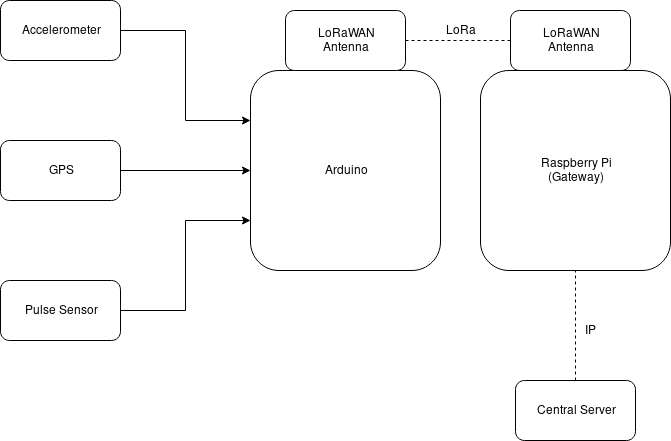
\includegraphics[width=0.3\textwidth]{images/Architecture.png}
		\caption[]{Schematic representation of the Architecture}
	\end{center}	
\end{figure}
\section{Weekly milestones}
A rough sketch of our weekly plan is as follows:

\begin{enumerate}
	\item Have the Raspberry Pi(Gateway) communicating with server.
	\item Have Arduino communicating with Raspberry Pi using LoRaWAN.
	\item Connect Accelerometer to Arduino and get its data on Server.
	\item Repeat step 4 for GPS and pulse sensor.
	\item Fit Components on the walker and preliminary tests
	\item Test the system, collect and plot data.
	\item Write the report
\end{enumerate}

\section{Strech Goals}
If we have addtional time, we can work on the following goals:
\begin{enumerate}
	\item Measure pressure applied on handles
	\item Analysis of collected data
	\item Measure durability/wear and tear
	\item Measure blood pressure
	\item Analyse gait
	\item Include a gsm adapter in the arduino, that way we can have bigger upload speeds, allowing us to have real-time updates which in turn would allow for use-cases of emergency situations and we would also be able to send video.
\end{enumerate}

\bibliography{ref}
\bibliographystyle{ieeetr}

\end{document}
